%%%%%%%%%%%%%%%%%%%%%%%%%%%%%%%%%%%%%%%%%%%%%%%%%%%%%%%%%%%%%%%%%%%%%%%%%%%%%%
% Document Settings and Command Definitions
%%%%%%%%%%%%%%%%%%%%%%%%%%%%%%%%%%%%%%%%%%%%%%%%%%%%%%%%%%%%%%%%%%%%%%%%%%%%%%

\documentclass[11pt]{article}

% Allow for T1 output font encoding and utf8 input font encoding
\usepackage[T1]{fontenc}
\usepackage[utf8]{inputenc}

% Get landscape pages in the document
\usepackage{pdflscape}

% Nice looking headers and footer
\usepackage{fancyhdr}

% Additional math packages
\usepackage[fleqn]{amsmath}
\usepackage{amssymb}
\usepackage{stmaryrd}

% Multirow command in tabular environemtns
\usepackage{multirow}

% Get text formatting for standard SI units
\usepackage{siunitx}

% Numbered lists and bullet points
\usepackage{enumitem}

% For including various types of files into the document  (.csv and .pdf)
\usepackage{pdfpages}
\usepackage{pgfplotstable}

% Packages for listing source code
\usepackage{listings}
\usepackage{minted}

% Package for flowcharts, graphs, and plots
\usepackage{tikz}
\usepackage{pgfplots}
\usetikzlibrary{arrows, positioning, shapes, calc}

% Page margin settings
\oddsidemargin0cm
\topmargin-2cm
\textwidth16.5cm
\textheight23.5cm

% Headers for each section of questions
\newcommand{\question}[2] {
    \noindent \begin{minipage}{\textwidth}
        \vspace{.25in} \hrule\vspace{0.5em}
        \noindent{\bf #1: #2} \vspace{0.5em}
        \hrule \vspace{.10in}
    \end{minipage} \\ \\
}

% Vertical space equivalent to a line of text
\newcommand{\linespace} {\vspace{\baselineskip}}

% Markers for each sub-part of a question
\newcommand{\subquestion}[1] {\noindent \textbf{#1}}
\renewcommand{\part}[1] {\vspace{.10in} {\bf (#1)}}

% Commands for fitting a figure to page (preserving its size), and scaling a
% figure to a page, which preserves its aspect ratio. The input should be a figure
\newcommand{\fittopage}[1] {
    \makebox[\textwidth]{
        #1
    }
}
\newcommand{\scaletopage}[1] {
    \hbox {
        \hspace{-5mm}
        \centerline{
            \resizebox{\paperwidth}{!}{
                #1
            }
        }
    }
}

% Useful aliases for name, andrew id, due date, assignment number, etc.
% These act as configurable settings on a per document basis, edit for each
\newcommand{\myname}{Brandon Perez and Rohit Banerjee}
\newcommand{\myandrew}{bmperez and rohitban}
\newcommand{\assignment}{Prelab 11}
\newcommand{\course}{18-348}
\newcommand{\mygroup}{Group C4}
\newcommand{\duedate}{April 10, 2015}

% Set up some block styles for drawing with tikz
\tikzstyle{node} = [circle, fill=blue!20, draw, font=\large\bfseries]
\tikzstyle{inout} = [font=\small\bfseries]
\tikzstyle{arrow} = [->, >=latex', shorten >=1pt, ->, >=stealth]
\tikzstyle{line} = [-]
\tikzstyle{empty} = [inner sep=0pt, minimum size=0pt]
\tikzstyle{arc} = [->, >=latex', short >=1pt, >=stealth, edge]
\tikzstyle{state} = [rounded rectangle, fill=blue!20, draw, align=center, font=\small\bfseries]

% Setup the default table style when importing from a csv file (full tabular environment)
\pgfplotstableset{
    col sep = comma,
    string type,
    column type = {|l},
    every last column/.style = {column type = {|l|}},
    every head row/.style = {before row = \hline},
    after row = \hline,
    % Bold all of the elements in the header row
    every head row/.append style = {
        typeset cell/.append code = {
             \ifnum\pgfplotstablecol=\pgfplotstablecols
                \pgfkeyssetvalue{/pgfplots/table/@cell content}{\textbf{##1}\\}%
            \else
                \pgfkeyssetvalue{/pgfplots/table/@cell content}{\textbf{##1}&}%
            \fi
        }
    },
}

% Set up a header on each page about the assignment
\pagestyle{fancyplain}
\lhead{\fancyplain{}{\textbf{\assignment}}}
\rhead{\fancyplain{}{\myname\\ \myandrew, \mygroup}}
\chead{\fancyplain{}{\course}}

%%%%%%%%%%%%%%%%%%%%%%%%%%%%%%%%%%%%%%%%%%%%%%%%%%%%%%%%%%%%%%%%%%%%%%%%%%%%%%
% Document
%%%%%%%%%%%%%%%%%%%%%%%%%%%%%%%%%%%%%%%%%%%%%%%%%%%%%%%%%%%%%%%%%%%%%%%%%%%%%%

\begin{document}
\medskip

% Create the title for the document
\thispagestyle{plain}
\begin{center}
	{\Large \course \ \assignment} \\
	\myname \\
	\myandrew, \mygroup \\
	\duedate \\
\end{center}

\question{Part 1}{Overall Project Description}
    \textbf{\underline{Project Description:}} \\

    Our project is to implement the game Snake on an LED matrix. The game will be controlled over the computer via serial communication,
    which will direct which direction the snake is moving. The game will end when the snake intersects with itself, allowing the snake
    to wrap around the board. Our reach goal for the project is to integrate a luminance sensor into the project to automatically adjust
    the brightness of the LED's based on the ambient lighting. Initially, this will be controlled by the on-board potentiometer. \\

    \noindent \textbf{\underline{Main Components of the Project:}}
    \begin{itemize}[noitemsep]
        \item Serial Communications
        \item PWM
        \item A/D
    \end{itemize}

    \noindent \textbf{\underline{Interrupt Service Routines:}}
    \begin{itemize}[noitemsep]
        \item Serial Communications Interrupt
        \item A/D Interrupt
    \end{itemize} \linespace

\question{Part 2}{Requirements}
    \textbf{\underline{System Inputs:}}
    \begin{enumerate}
        \item pauseButton
        \begin{itemize}[nolistsep, noitemsep, label=--]
            \item Indicates to pause the game. Values are PRESSED and UNPRESSED. This will be from a push button on
            the project board.
        \end{itemize}
        \item brightnessReady
        \begin{itemize}[nolistsep, noitemsep, label=--]
            \item Indicates that a new brightness level for the LED's is ready. This is a binary value. This will
            come in the form of an A/D interrupt.
        \end{itemize}
        \item brightness
        \begin{itemize}[nolistsep, noitemsep, label=--]
            \item Indicates the brightness level of the LED's. This is an integral value. This will be an input from
            the A/D converter.
        \end{itemize}
        \item directionReady
        \begin{itemize}[nolistsep, noitemsep, label=--]
            \item Indicates that a new direction for the snake is ready. This is a binary value.
            This will come in the form of a Serial Communications interrupt.
        \end{itemize}
        \item direction
        \begin{itemize}[nolistsep, noitemsep, label=--]
            \item Indicates the direction to move the snake in. Values are LEFT, RIGHT, UP, DOWN. This will
            be an input from the Serial Communication with the computer.
        \end{itemize}
    \end{enumerate} \linespace

    \noindent \textbf{\underline{System Outputs:}}
    \begin{enumerate}
        \item snakeBoard
        \begin{itemize}[nolistsep, noitemsep, label=--]
            \item Indicates the current state of the snake game. This is a 2D array where each value represents
            the state of that LED. The values for each element are OFF, FOOD, or SNAKE.
        \end{itemize}
        \item boardBrightness
        \begin{itemize}[nolistsep, noitemsep, label=--]
            \item Indicates the current brightness of the LED's on the snake game. This is an integral value.
        \end{itemize}
        \item score
        \begin{itemize}[nolistsep, noitemsep, label=--]
            \item Indicates the current score of the game, which is the number of food pieces consumed by the snake.
            This will also be used to track the length of the snake, as it grows by one every time food is consumed.
        \end{itemize}         
    \end{enumerate} \linespace

    \noindent \textbf{\underline{Internal State Variables:}}
    \begin{enumerate}[noitemsep]
        \item gameState
        \begin{itemize}[nolistsep, noitemsep, label=--]
            \item Indicates the current state of the snake game. Values are PLAYING, PAUSED, and GAMEOVER.
        \end{itemize}
        \item snakeHead
        \begin{itemize}[nolistsep, noitemsep, label=--]
            \item Indicates the current position of the head of the snake. This is an integral value.
        \end{itemize}
        \item snakeDirection
        \begin{itemize}[nolistsep, noitemsep, label=--]
            \item Indicates if the current direction that the snake is moving. Values are RIGHT, LEFT, UP, and DOWN.
        \end{itemize}
        \item foodPosition
        \begin{itemize}[nolistsep, noitemsep, label=--]
            \item Indicates the current position of the food on the board. This is an integral value.
        \end{itemize}           
    \end{enumerate}

    \noindent \textbf{\underline{Requirements:}} \\ \\
    \begin{tabular}{rl}
        \indent & R1. Pressing PB1 shall pause the game \\
        & R2. Pressing the left arrow key shall cause the snake to turn left. \\
        & R3. Pressing the right arrow key shall cause the snake to turn right. \\
        & R4. Pressing the up arrow key shall cause the snake to turn upwards. \\
        & R5. Pressing the down arrow key shall cause the snake to turn downwards. \\
        & R6. The game shall end if the snake collides with itself. \\
        & R7. The LCD display shall display the current score. \\
        & R8. Adjusting the analog input shall change the brightness of the LED display. \\
        & R9. The snake running into the food shall increment the score and generate a new \\ 
        & piece of food on the board. \\         
        & R10. The snake running into the food shall increase the snake's length by 1.
    \end{tabular} \\

\question{Part 4}{State Chart and Requirement Traceability Table} \vspace{-20mm}
    \pagebreak
    \begin{landscape}
        \makebox[\paperwidth]{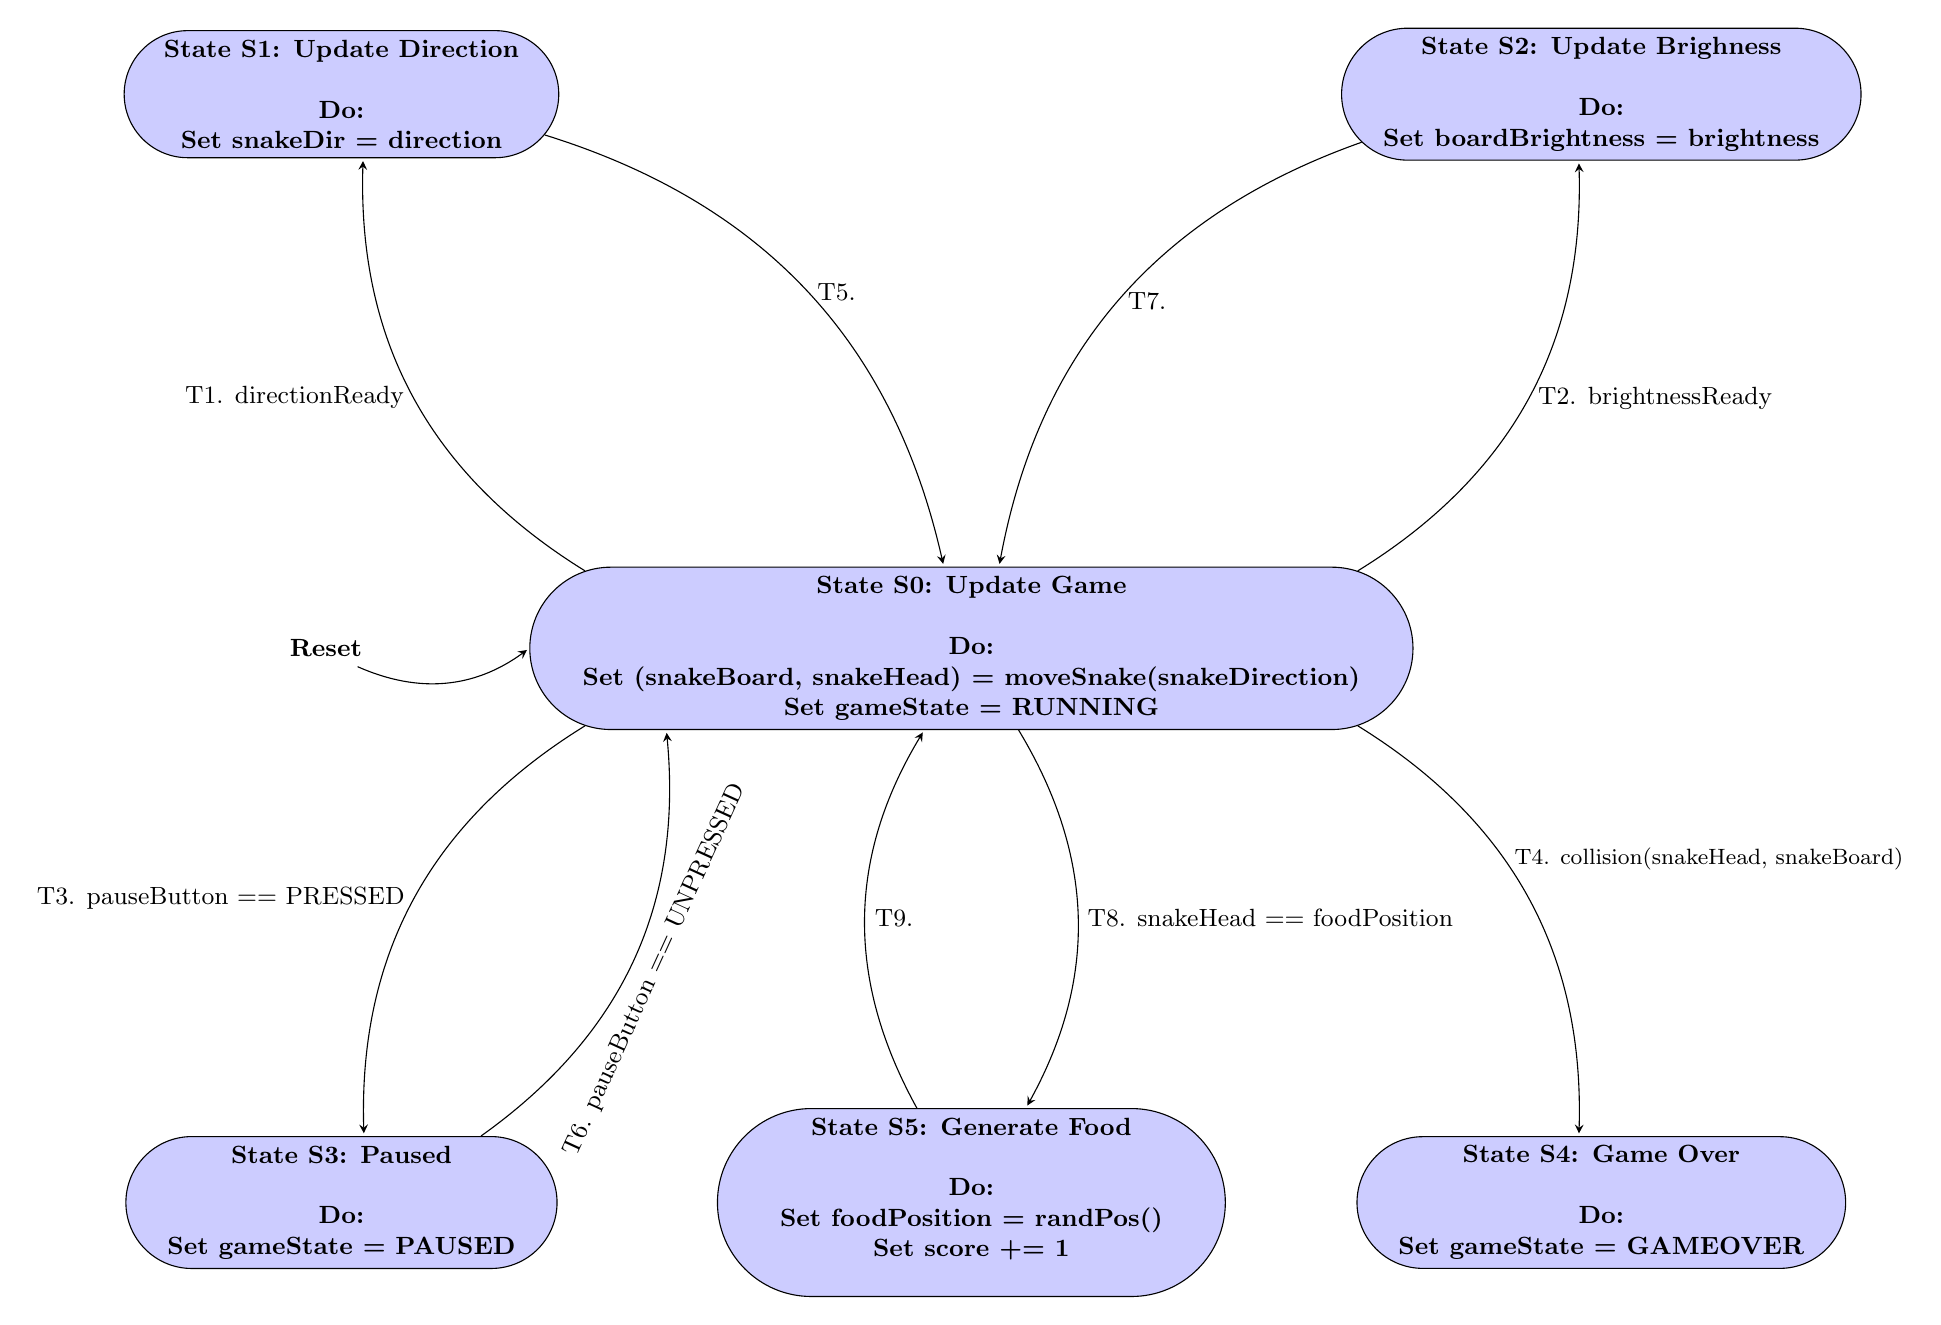
\begin{tikzpicture}
            % The states
            \node[state] (update_game) at (current bounding box.center)
                {State S0: Update Game\\\\
                    Do:\\
                    Set (snakeBoard, snakeHead) = moveSnake(snakeDirection)\\
                    Set gameState = RUNNING};
            \node[state] (update_direction) at ($(update_game.north)+(-8,6)$)
                {State S1: Update Direction\\\\
                    Do:\\
                    Set snakeDir = direction};
            \node[state] (update_brightness) at ($(update_game.north)+(8,6)$)
                {State S2: Update Brighness\\\\
                    Do:\\
                    Set boardBrightness = brightness};
            \node[state] (pause) at ($(update_game.south)+(-8,-6)$)
                {State S3: Paused\\\\
                    Do:\\
                    Set gameState = PAUSED};
            \node[state] (over) at ($(update_game.south)+(8,-6)$)
                {State S4: Game Over\\\\
                    Do:\\
                    Set gameState = GAMEOVER};
            \node[state] (consume_food) at ($(update_game.south)+(0,-6)$)
                {State S5: Generate Food\\\\
                    Do:\\
                    Set foodPosition = randPos()\\
                    Set score += 1\\};

            % The transitions
            \node[inout] (reset) [left = 2 of update_game.west] {Reset};

            \draw[arrow] (reset) edge [bend right] (update_game.west);
            \draw[arrow] (update_game) edge [bend left] node [anchor=east, font=\small]
                {T1. directionReady}
                (update_direction);
            \draw[arrow] (update_game) edge [bend right] node [anchor=west, font=\small]
                {T2. brightnessReady}
                (update_brightness);
            \draw[arrow] (update_game) edge [bend right] node [anchor=east, font=\small]
                {T3. pauseButton == PRESSED}
                (pause);
            \draw[arrow] (update_game) edge [bend left] node [anchor=west, font=\footnotesize, yshift=5mm, xshift=-3mm]
                {T4. collision(snakeHead, snakeBoard)}
                (over);
            \draw[arrow] (update_game) edge [bend left] node [anchor=west, font=\small]
                {T8. snakeHead == foodPosition}
                (consume_food);
            \draw[arrow] (update_direction) edge [bend left] node [anchor=west, font=\small]
                {T5.}
                (update_game);
            \draw[arrow] (update_brightness) edge [bend right] node [anchor=west, font=\small]
                {T7.}
                (update_game);
            \draw[arrow] (pause) edge [bend right] node [anchor=west, xshift=-27mm, yshift=-3mm, sloped, font=\small]
                {T6. pauseButton == UNPRESSED}
                (update_game.195);
            \draw[arrow] (consume_food) edge [bend left] node [anchor=west, font=\small]
                {T9.}
                (update_game);
        \end{tikzpicture}}
    \end{landscape}
%
    \pagebreak
    \noindent \textbf{\underline{State Chart Traceability Table:}} \\ \\
    \scaletopage{\pgfplotstabletypeset[
        every col no 1/.append style = {column type = {|l}},
        every col no 1/.append style = {column type = {|l}}
    ]{tables/q4.csv}} \\ \\ \\

\question{Part 5}{Scheduling}
    Scheduling method: Cyclic executive main loop with prioritized cooperative context switching. \\

    \noindent \textbf{\underline{Tasks and Priority:}} \\ \\
    \pgfplotstabletypeset[
        every col no 1/.append style = {column type = {|l}},
        every col no 1/.append style = {column type = {|l}}
    ]{tables/q5.csv} \\ \\

    The persistence of vision effect for humans is sustained around about 10 ms, so we decided to make the game
    update run at this rate, because we will be serially driving individual LED's on the matrix. We decided to have the 
    updates to the direction and the brightness to run every 100 ms the as human reaction time is about 215 ms, and
    we leave some margin for error. \\

    \noindent \textbf{\underline{Task Durations:}} \\ \\
    \begin{tabular}{rll}
        \indent & Update direction &= (10 bits / 9600 baud) = 1.04 ms \\
        & Update brightness &= (8 bits * 1bit/cycle) / (8MHz) = \SI{1.00}{\micro\second} \\
    \end{tabular} \\ \\

    \noindent \textbf{\underline{Game Update Duration:}} \\ \\
    \begin{tabular}{rll}
        \indent & Assume that the LED matrix is an 8x8 array	& \\
        & Worst case conditional cycles &= 64*3 \\
        & Worst case memory cycles &= 64*4 \\
        & Worst case register increment cycles &= 64 \\
        & Worst case LCD matrix update &= 64*4 + 64 \\
        & Total time taken &= Summation of above value / 8MHz \\
        & &= 0.104 ms
    \end{tabular} \\ \\

    In our scheduling method, we schedule the brightness update before the direction update as it has a shorter runtime. \\ \\

\question{Part 6}{Watchdog/COP}
    \indent The program shall use a watch dog that is kicked every 102 ms as in the worst case we have to
    wait 100 ms and then execute all three of our tasks. In the event of a watchdog reset, the
    program shall display an error message on the LCD display. \\ \\

\question{Part 7.1}{White Box Testing}
    \textbf{\underline{White Box Tests:}} \\ \\
    \fittopage{\pgfplotstabletypeset[
        col sep = semicolon,
        every col no 0/.append style = {column type = {|l}},
        every col no 0/.append style = {column type = {|l}}
    ]{tables/q7.1.1.csv}} \\ \\

    \noindent \textbf{\underline{White Box Test Traceability:}} \\ \\
    \pgfplotstabletypeset[
        every col no 0/.append style = {column type = {|l}},
        every col no 0/.append style = {column type = {|l}}
    ]{tables/q7.1.2.csv} \\ \\ \\

\question{Part 7.2}{Black Box Testing}
    \textbf{\underline{Black Box Tests:}} \\ \\
    \scaletopage{\pgfplotstabletypeset[
        every col no 0/.append style = {column type = {|l}},
        every col no 0/.append style = {column type = {|l}}
    ]{tables/q7.2.1.csv}} \\ \\ \\

    \noindent \textbf{\underline{Black Box Test Traceability:}} \\ \\
    \pgfplotstabletypeset[
        every col no 0/.append style = {column type = {|l}},
        every col no 0/.append style = {column type = {|l}}
    ]{tables/q7.2.2.csv} \\ \\ \\

\question{Part 8}{Hardware}
    \textbf{\underline{List of Hardware Components:}}
    \begin{enumerate}[noitemsep]
        \item Texas Instruments OPT101P - IC Photodiode and Amplifier (1) (Will be acquired by us)
        \item LS138 - Decoder/Demultiplexer (2)
        \item LEDs (64)
        \item Current-Limiting Resistors (8)
    \end{enumerate} \linespace

    \noindent \textbf{\underline{Hardware Schematic:}} \\ \\
    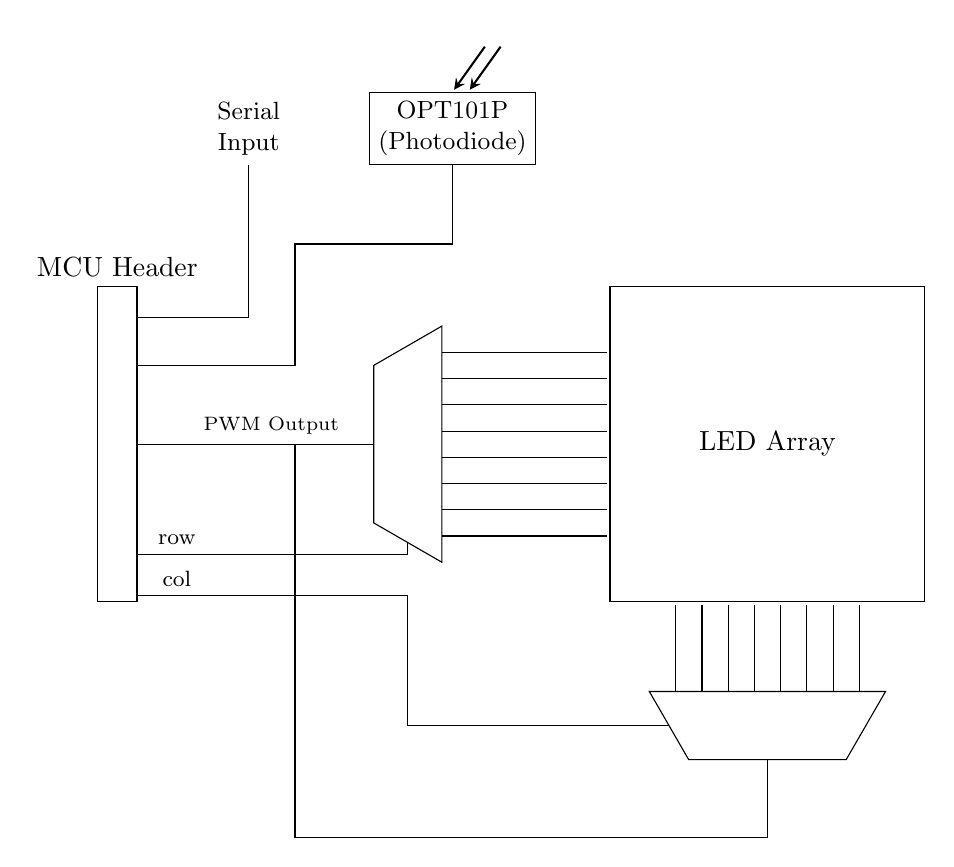
\begin{tikzpicture}
        % Chip header
        \node[rectangle, draw, minimum width=5mm, minimum height=40mm, label=MCU Header] (pin_header) at (0,0) {};

        % Demultiplexer 1
        \coordinate (d1) at ($(pin_header.east)+(3,1)$);
        \draw (d1) -- ++(270:2) coordinate (A1) -- ++(330:1) coordinate (B1) -- ++(90:3) coordinate (C1) -- ++(210:1) -- cycle;

        % LED Array
        \node[rectangle, draw, minimum width=40mm, minimum height=40mm] (led_array) at ($(d1)+(5,-1)$) {LED Array};

        % Demultiplexer 2
        \coordinate (d2) at ($(led_array.south)+(-1,-2)$);
        \draw[rotate=90] (d2) -- ++(270:2) coordinate (A2) -- ++(330:1) coordinate (B2) -- ++(90:3) coordinate (C2) -- ++(210:1) -- cycle;

        % Luminence Sensor
        \node[rectangle, draw, font=\small, align=center] (sensor) at ($(pin_header.north east)+(4,2)$) {OPT101P\\(Photodiode)};
        \node[inout] (l1) at ($(sensor.north)+(0.5,0.7)$) {};
        \node[inout] (l2) at ($(sensor.north)+(0.7,0.7)$) {};
        \draw[arrow, line width=0.75pt] (l1) -- (sensor.north);
        \draw[arrow, line width=0.75pt] (l2) -- ($(sensor.north)+(0.2,0)$);

        % Serial input
        \node[rectangle, font=\small, align=center] (serial) [left = 1 of sensor.west] {Serial\\Input};

        % Pin header Connections
        \draw[line] (pin_header.east) node [above, font=\scriptsize, xshift=17mm] {PWM Output} -- ($(d1)+(0,-1)$);
        \draw[line] (pin_header.east) -- ++(2,0) -- ++(0,-5) -- ++(6,0) -- ++(0,1);
        \draw[line] ($(pin_header.south east)!0.15!(pin_header.north east)$) node [above, font=\footnotesize, xshift=5mm] {row} -| ($(A1)!0.50!(B1)$);
        \draw[line] ($(pin_header.south east)!0.02!(pin_header.north east)$) node [above, font=\footnotesize, xshift=5mm] {col} -| ($(A1)!0.50!(B1)+(0,-2)$) |- ($(d2)!0.50!(C2)$);
        \draw[line] ($(pin_header.south east)!0.90!(pin_header.north east)$) -| (serial);
        \draw[line] (sensor.south) -- ++(0,-1) -- ++(-2,0) |- ($(pin_header.south east)!0.75!(pin_header.north east)$);

        % Demultiplexer connections
        \draw[line] ($(B1)!0.111!(C1)$) -- ++(2.1,0);
        \draw[line] ($(B1)!0.222!(C1)$) -- ++(2.1,0);
        \draw[line] ($(B1)!0.333!(C1)$) -- ++(2.1,0);
        \draw[line] ($(B1)!0.444!(C1)$) -- ++(2.1,0);
        \draw[line] ($(B1)!0.555!(C1)$) -- ++(2.1,0);
        \draw[line] ($(B1)!0.666!(C1)$) -- ++(2.1,0);
        \draw[line] ($(B1)!0.777!(C1)$) -- ++(2.1,0);
        \draw[line] ($(B1)!0.888!(C1)$) -- ++(2.1,0);

        \draw[line] ($(B2)!0.111!(C2)$) -- ++(0,1.1);
        \draw[line] ($(B2)!0.222!(C2)$) -- ++(0,1.1);
        \draw[line] ($(B2)!0.333!(C2)$) -- ++(0,1.1);
        \draw[line] ($(B2)!0.444!(C2)$) -- ++(0,1.1);
        \draw[line] ($(B2)!0.555!(C2)$) -- ++(0,1.1);
        \draw[line] ($(B2)!0.666!(C2)$) -- ++(0,1.1);
        \draw[line] ($(B2)!0.777!(C2)$) -- ++(0,1.1);
        \draw[line] ($(B2)!0.888!(C2)$) -- ++(0,1.1);
    \end{tikzpicture} \linespace \linespace

\question{Part 9}{Acceptance Test Plan}
    \noindent \textbf{\underline{Acceptance Procedure:}}
    \begin{itemize}[noitemsep]
        \item The snake shall move according to arrow key presses on the computer.
        \item There shall be no visible delay in the direction change of the snake.
        \item The user shall be able to play the game for at least 30s continuously without any interruptions (barring a game over).
        \item If a food cell is collected, the length of the snake shall increase by 1 unit and the score counter shall be incremented by 1.
        \item If the light sensor is implemented, shining a torchlight or placing the board in darkness shall cause the led intensity to be adjusted (decreased or increased respectively).
        \item If the light sensor is not implemented, adjusting the on-board potentiometer shall cause the LEDs to increase and decrease intensity.
        \item None of the above procedures shall cause a watchdog reset error to be displayed on the LCD display.
    \end{itemize}

\end{document}
